\documentclass[11pt,a4paper]{article}
\usepackage[margin=1in]{geometry}
\usepackage[T1]{fontenc}
\usepackage[utf8]{inputenc}
\usepackage{lmodern}
\usepackage{hyperref}
\usepackage{enumitem}
\usepackage{xurl}
\usepackage{tikz}
\usepackage{float}
\usetikzlibrary{arrows.meta, positioning, shapes.geometric}
\hypersetup{colorlinks=true,linkcolor=blue,urlcolor=blue}
\newcommand{\codepath}[1]{\path{#1}}
\tikzset{box/.style={rectangle,draw,rounded corners,align=center,inner sep=3pt,minimum width=36mm},decision/.style={diamond,draw,aspect=2.1,align=center,inner sep=2pt},line/.style={-Latex}}

\title{Phase-1 Deliverable: Time and Windowing}
\author{SIT Engine Architecture}
\date{\today}

\begin{document}
\maketitle

\section{Technical Description}
This deliverable defines the canonical monotonic time model and fixed-window slicing used across all sources. It guarantees boundary-correct overlap handling using half-open interval semantics.

\section{Implementation Fulfillment}
Implemented in \codepath{Phase-1/sit_engine_phase1.py} via \texttt{split\_interval\_into\_windows}. Exact boundary handling uses \texttt{floor((end\_us - 1e-9)/window\_us)}. Tests are encoded in \codepath{Phase-1/tests/check_invariants.py} through \texttt{check\_partial\_expected\_resident\_us} and \texttt{check\_exact\_boundary}, executed by \codepath{Phase-1/tests/run_golden_suite.py}.

\section{Design \& Architecture}
All intervals are processed as $[start,end)$ and decomposed into positive overlap fragments per window. This keeps aggregation deterministic and prevents double-counting at boundaries.

\subsection*{Function Flowchart}
\begin{figure}[H]
\centering
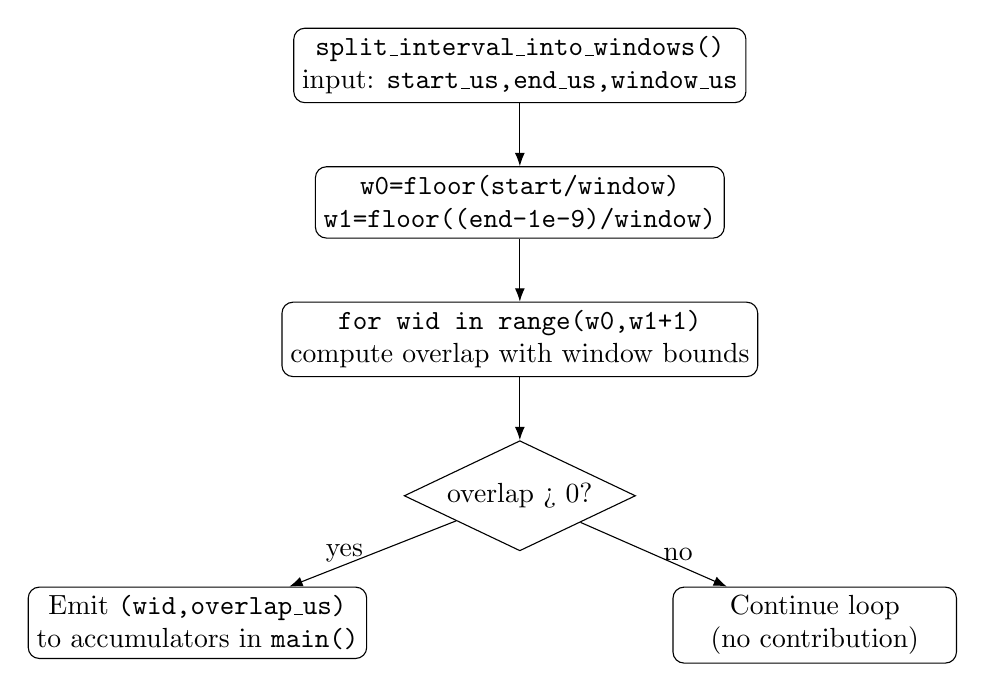
\begin{tikzpicture}[node distance=8mm and 12mm]
\node[box] (a) {\texttt{split\_interval\_into\_windows()}\\input: \texttt{start\_us,end\_us,window\_us}};
\node[box, below=of a] (b) {\texttt{w0=floor(start/window)}\\\texttt{w1=floor((end-1e-9)/window)}};
\node[box, below=of b] (c) {\texttt{for wid in range(w0,w1+1)}\\compute overlap with window bounds};
\node[decision, below=of c] (d) {overlap > 0?};
\node[box, below left=of d] (e1) {Emit \texttt{(wid,overlap\_us)}\\to accumulators in \texttt{main()}};
\node[box, below right=of d] (e2) {Continue loop\\(no contribution)};
\draw[line] (a) -- (b);
\draw[line] (b) -- (c);
\draw[line] (c) -- (d);
\draw[line] (d) -- node[left]{yes} (e1);
\draw[line] (d) -- node[right]{no} (e2);
\end{tikzpicture}
\caption{Time and Windowing Function Flow}
\end{figure}

\end{document}
